
%(BEGIN_QUESTION)
% Copyright 2010, Tony R. Kuphaldt, released under the Creative Commons Attribution License (v 1.0)
% This means you may do almost anything with this work of mine, so long as you give me proper credit

En vannelektrolysekrets omformer AC til DC og bruker en {\it shuntmotstand} for å måle strøm gjennom elektrolysecellene:

$$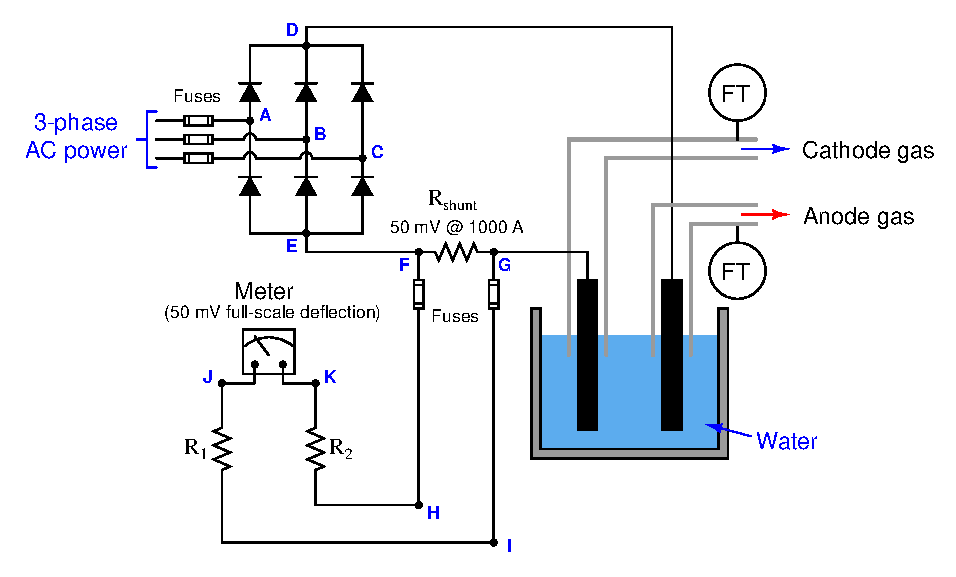
\includegraphics[width=15.5cm]{i00622x01.eps}$$

Operatøren melder at gassproduksjonen plutselig har stoppet, men strømmåleren viser over 1000 A (``pegget'' full skala). Første steg er å måle spenning mellom punkt I og H, og multimeteret viser langt over 50 mV DC.

Vurder sannsynlighet for hver oppgitt feil. Vurder én og én feil (ingen samtidige feil), og avgjør om feilen alene kan forklare {\it alle} målinger og symptomer.

% No blank lines allowed between lines of an \halign structure!
% I use comments (%) instead, so that TeX doesn't choke.

$$\vbox{\offinterlineskip
\halign{\strut
\vrule \quad\hfil # \ \hfil & 
\vrule \quad\hfil # \ \hfil & 
\vrule \quad\hfil # \ \hfil \vrule \cr
\noalign{\hrule}
%
% First row
{\bf Feil} & {\bf Mulig} & {\bf Umulig} \cr
%
\noalign{\hrule}
%
% Another row
$R_1$ eller $R_2$ åpen feil &  &  \cr
%
\noalign{\hrule}
%
% Another row
$R_{shunt}$ åpen feil &  &  \cr
%
\noalign{\hrule}
%
% Another row
En metersikring utløst &  &  \cr
%
\noalign{\hrule}
%
% Another row
En AC-forsyningssikring utløst &  &  \cr
%
\noalign{\hrule}
%
% Another row
$R_1$ eller $R_2$ kortsluttet &  &  \cr
%
\noalign{\hrule}
%
% Another row
$R_{shunt}$ kortsluttet &  &  \cr
%
\noalign{\hrule}
%
% Another row
Brudd i leder mellom G og katode &  &  \cr
%
\noalign{\hrule}
%
% Another row
Brudd i leder mellom D og anode &  &  \cr
%
\noalign{\hrule}
} % End of \halign 
}$$ % End of \vbox

Identifiser også hvilke gasstyper du forventer fra henholdsvis anode og katode, og et godt valg av flowmåleteknologi for hver gass.

\vfil

\underbar{file i00622}
\eject
%(END_QUESTION)





%(BEGIN_ANSWER)

Dette er en vurdert oppgave -- ingen svar eller hint oppgis!

%(END_ANSWER)





%(BEGIN_NOTES)

Hvis gassproduksjon stopper, betyr det at normal strøm gjennom elektrolysecellen er kraftig redusert. Vi leter derfor etter feil som gir lav celle-strøm men høy indikert strøm. Av feilene listet er det bare én som forklarer begge symptomer:

% No blank lines allowed between lines of an \halign structure!
% I use comments (%) instead, so that TeX doesn't choke.

$$\vbox{\offinterlineskip
\halign{\strut
\vrule \quad\hfil # \ \hfil & 
\vrule \quad\hfil # \ \hfil & 
\vrule \quad\hfil # \ \hfil \vrule \cr
\noalign{\hrule}
%
% First row
{\bf Feil} & {\bf Mulig} & {\bf Umulig} \cr
%
\noalign{\hrule}
%
% Another row
$R_1$ eller $R_2$ åpen feil &  & $\surd$ \cr
%
\noalign{\hrule}
%
% Another row
$R_{shunt}$ åpen feil & $\surd$ &  \cr
%
\noalign{\hrule}
%
% Another row
En metersikring utløst &  & $\surd$ \cr
%
\noalign{\hrule}
%
% Another row
En AC-forsyningssikring utløst &  & $\surd$ \cr
%
\noalign{\hrule}
%
% Another row
$R_1$ eller $R_2$ kortsluttet &  & $\surd$ \cr
%
\noalign{\hrule}
%
% Another row
$R_{shunt}$ kortsluttet &  & $\surd$ \cr
%
\noalign{\hrule}
%
% Another row
Brudd i leder mellom G og katode &  & $\surd$ \cr
%
\noalign{\hrule}
%
% Another row
Brudd i leder mellom D og anode &  & $\surd$ \cr
%
\noalign{\hrule}
} % End of \halign 
}$$ % End of \vbox

Hydrogen forventes ved katode, oksygen ved anode. En god flowteknologi er {\it termisk massestrøm} for begge gasser, med lav kost og lav følsomhet for sammensetningsendring.

\vskip 20pt \vbox{\hrule \hbox{\strut \vrule{} {\bf Virtuell feilsøking} \vrule} \hrule}

Oppgaven egner seg godt for virtuell feilsøking: definer en feil, presenter symptomer, la studentene foreslå tester, og oppgi resultat for hver test.

%INDEX% Prosess: elektrolyse av vann
%INDEX% Feilsøkingsrepetisjon: elektriske kretser

%(END_NOTES)

